\documentclass{standalone}
\usepackage{tikz}

\begin{document}

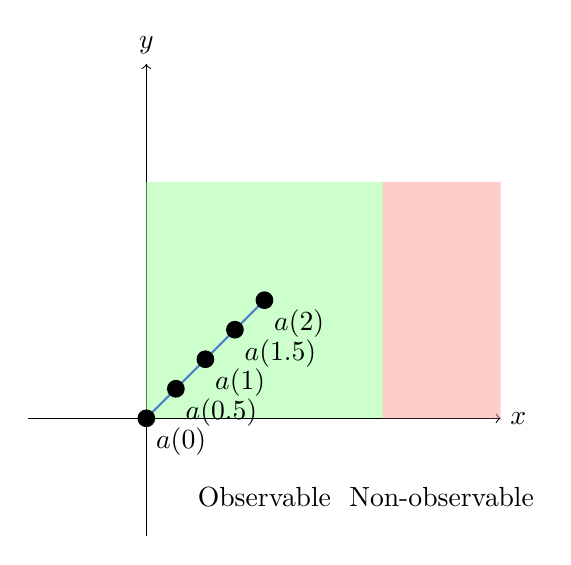
\begin{tikzpicture}[scale=1.5]
    % Axes
    \draw[->] (-1,0) -- (3,0) node[right] {$x$};
    \draw[->] (0,-1) -- (0,3) node[above] {$y$};

    % Trajectory
    \draw[thick, blue] plot[domain=0:2, samples=100] (\x*0.5, \x*0.5);

    % Observable region (green)
    \fill[green!40!white, opacity=0.5] (0,0) rectangle (2,2);
    
    % Non-observable region (red)
    \fill[red!40!white, opacity=0.5] (2,0) rectangle (3,2) |- cycle;

    % Points on the trajectory
    \foreach \x in {0, 0.5, 1, 1.5, 2} {
        \filldraw[black] (\x*0.5, \x*0.5) circle (2pt) node[below right] {$a(\x)$};
    }

    % Labels
    \node at (1, -0.5) [below] {Observable};
    \node at (2.5, -0.5) [below] {Non-observable};
\end{tikzpicture}

\end{document}